\documentclass{article}
\usepackage[margin=1in]{geometry}
\usepackage{amsmath,amsthm,amssymb}
\usepackage{bbm,enumerate,mathtools}
\usepackage{tikz,pgfplots}
\usepackage{chessboard}
\usepackage[hidelinks]{hyperref}
\usepackage{multicol} % Problem 35

\newenvironment{question}{\begin{trivlist}\item[\textbf{Question.}]}{\end{trivlist}}
\newenvironment{note}{\begin{trivlist}\item[\textbf{Note.}]}{\end{trivlist}}
\newenvironment{references}{\begin{trivlist}\item[\textbf{References.}]}{\end{trivlist}}
\newenvironment{related}{\begin{trivlist}\item[\textbf{Related.}]\end{trivlist}\begin{enumerate}}{\end{enumerate}}


\begin{document}
\rating{3}{1}
Call $s$ an ``initial permutable'' string if for every initial substring of
odd length, the first half of the string is a permutation of the second half.
\begin{figure}[!h]
  \centering
  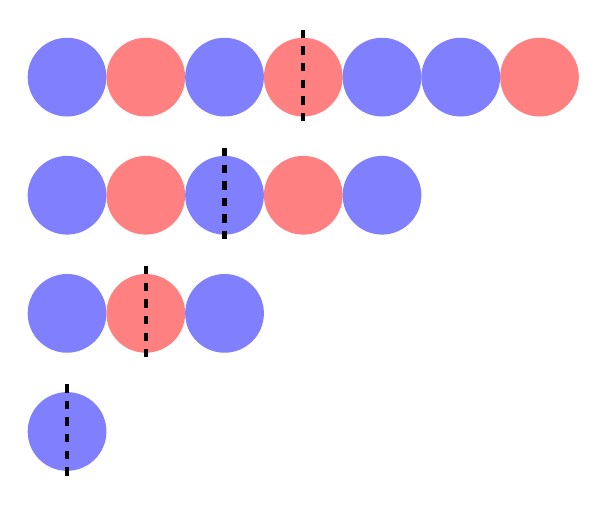
\begin{tikzpicture}
    \foreach \x/\y/\c in {
      1/1/blue, 2/1/red, 3/1/blue, 4/1/red, 5/1/blue, 6/1/blue, 7/1/red,
      1/-0.5/blue, 2/-0.5/red, 3/-0.5/blue, 4/-0.5/red, 5/-0.5/blue,
      1/-2/blue, 2/-2/red, 3/-2/blue,
      1/-3.5/blue} {
      \fill[\c!50] (\x, \y) circle (0.5);
    }
    \draw[ultra thick, dashed] (4,1.6)--(4,0.4);
    \draw[ultra thick, dashed] (3,0.1)--(3,-1.1);
    \draw[ultra thick, dashed] (2,-1.4)--(2,-2.6);
    \draw[ultra thick, dashed] (1,-2.9)--(1,-4.1);
  \end{tikzpicture}
  % \begin{align*}
  %   1\ 0\ 1\ 0\ 1\ 1\ 0 &\rightarrow 1\ 0\ 1\ 0\ \sim 0\ 1\ 1\ 0\\
  %   1\ 0\ 1\ 0\ 1 &\rightarrow 1\ 0\ 1 \sim 0\ 1\ 0\\
  %   1\ 0\ 1 &\rightarrow 1\ 0 \sim 0\ 1\\
  %   1 &\rightarrow 1 \sim 1
  % \end{align*}
  \caption{
    ``BRBRBBR'' is an example of an initial permutable string. Because each
    initial odd substring (the string itself, ``BRBRB'', ``BRB'', and ``B'')
    has the property that the first half of the string is a rearrangement of
    second half.
  }
\end{figure}

\begin{question}
  What is the growth of $a_2(n)$, the number of initial permutable strings of
  length $2n - 1$ over a $2$-letter alphabet?
\end{question}
\begin{related}
  \item Can this be generalized to a $k$-letter alphabet?
\end{related}
\begin{references}
  \item \url{http://oeis.org/A297789}
\end{references}
\end{document}
